\documentclass[colorlinks=true,pdfstartview=FitV,linkcolor=blue,
            citecolor=red,urlcolor=magenta]{ligodoc}

\usepackage{graphicx}
\usepackage{amssymb}
\usepackage{amsmath}
\usepackage{longtable}
\usepackage{rotating}
\usepackage[usenames,dvipsnames]{color}
\usepackage{fancyhdr}
\usepackage{subfigure}
\usepackage{hyperref}
\usepackage{mathtools}

\ligodccnumber{T}{17}{00198}{}{v1}% \ligodistribution{AIC, ISC}

\setlength\parindent{24pt}

\title{Online Detector Characterization using Neural Networks}

\author{Roxana Popescu}

\begin{document}

\section{Introduction} 

\indent

\par The data obained from LIGO has noise that comes from many sources. In order to be able to better distinguish signals from the noise, it is important to characterize the type of noise observed. Machine learning algorthms can be used to look for patterns within the data and to classify the data into different categories.

\par There are many sensors at the LIGO detectors that measure sources of noise. For example, there are several stations at each LIGO detector that measure seismic noise in different frequency channels in each of the X,Y, and Z directions. Within the data, there are different types of seismic noise such as earthquakes and anthropogenic noise.  

\par In order to sort data, machine learning algorithms can use one of two approaches: classification or clustering. Classification algorithms search the data and sort the data into already defined categories. Clustering algorithms look for relationships within the data to create categories into which the data is sorted. Classification algorithms are part of supervised learning since the computer determines the structure of the data from data that is already provided. Clustering algorithms are part of unsupervised learning since the computer determines the structure of the data without any previous information. Clustering algorithms can be used to characterize the noise by identifying common characteristics within the noise and the clustering algorithms can further help with classification. \cite{Citation1}

\par Neural networks can be used to find relationships between the inputed data by using hidden layers of connections within the data. Recurrent neural networks are neural networks that use loops within them so that previous information can be retained. \cite{Citation1}

\section{Objectives}

\indent

\par The aim of this project is to characterize different sources of noise from LIGO using machine learning algorithms. First I  will test clustering algorithms on seismic data, and then implement a neural network to sort through the seismic noise data, as well as other noise data.

\section{Clustering Algorithms}

\subsection{K-means Clustering}

\indent

\par The k-means clustering algorithm creates clusters by separating data points into k number of groups. The value of k is inputted into the algorithm. The clusters are determined by minimizing the inertia, or the within-cluster sum-of-squares. The inertia is a measure of how coherent the clusters are. By minimizing the intertia, the algorithm tries to minimize the difference between the mean value of a cluster and the values of points in the cluster. If a set of n samples x are inputted, the algorithm divides the samples into k clusters C. Each cluster is described by its mean \(u_j\), or centroid. The interia of a cluster is caluclated by the following expression:

\[\sum_{i=0}^{n} \min_{\mu_j \in  C}(\|x_j-\mu_i\|^2)\]

\par The inertia is not normalized, but lower values are better and zero is the optimum value. The inertia assumes that the clusters are convex and isotropic, and would not work well to cluster irregular or elongated clusters. \cite{Citation2} 

\subsection{DBSCAN Clustering}

\indent

\par The DBSCAN clustering algorithm creates clusters out of areas in the data of higher density. Unlike kmeans, it does not consider clusters to have any particular shapes, and the algorithm determines the number of clusters based on inputted parameters. Core samples are points that are in areas of high densities. The algorithm creates clusters around core samples so that the clusters consist of core samples, and non-core samples that are close to the core samples. The core samples are determined by two input parameters, the minimum samples and a specified distance, $\varepsilon$. A point is in the $\varepsilon$-neighborhood if the distance d from a point p to a point q is within a radius of of $\varepsilon$, as determined below: 

\[N_\varepsilon(p):\{q|d(p,q) \leq \varepsilon\}\]

\par High density areas have the minimum sample of values within the $\varepsilon$-neighborhood. By increasing the number of minimum samples, and decreasing the distance, $\varepsilon$, a cluster's density is increased. \cite{Citation2}\cite{Citation3}

\subsection{Agglomerative Clustering}

\indent

\par Agglomerative clustering is a type of hierarchical clustering algorithm. Hierarchical clustering builds clusters by merging and splitting clusters many times. Agglomerative clustering works by initially giving each data point its own cluster and then merging the clusters until the inputed number of clusters is reached. \cite{Citation2}

\subsection{Evaluating Clustering Algorithms}

\subsubsection{Calinsky Harabaz Index}

\indent

\par The Calinsky-Harabaz index is a method used to evaluate how well clustering algorithms work, that does not require input of external data. The Calinsky-Harabaz score is calculated by finding the ratio of the between-clusters dispersion mean to the within-cluster dispersion mean. This ratio is calculated as follows:

\[s(k) = \frac{Tr(B_k)}{Tr(W_k)}\times\frac{N-k}{k-1}\]

\par Where k is the number of clusters, \(B_k\) is the between group dispersion matrix, \(W_k\) is the within group dispersion matrix and N is the number of data points. \(W_k\) and  \(B_k\) are defined by:

\[W_k = \sum_{q=1}^{k} \sum_{x \in C_q} (x-c_q)(x-c_q)^T\]

\[B_k = \sum_{q} n_q (c_q-c)(c_q-c)^T\]

\par Where \(C_q\) is the number of set points in cluster q, \(c_q\) is the center of cluster q, c is the center of the clusters, and \(n_q\) is the number of points in cluster q. \cite{Citation2} 

\subsubsection{Comparing Clusters to Earthquake Times}

\indent 

\par Another way to evaluate how well the clustering algorithms work is to add up the cluster labels that occur five  minutes before and after an earthquake Rayleigh wave arrives, to add up the total amount of cluster labels, and for each individual cluster to divide the number of cluster labels that appear near the earthquake by the total number of cluster labels. For each cluster k, the earthquake comparison score, E(k) can be determined by:

\[E(k) = \frac{N_e}{N_t}\]

Where \(N_e\) is the number of cluster labels five minutes before and after an earthquake, and \(N_t\) is the total number of cluster labels. If a cluster corresponds to the presence of an earthquake then it will have a high percentage of its cluster labels present near an earthquake.  

\section{Current Progress}

\indent 

\par I have written a script that determines how well clusters determined by clustering algorithms correspond to recorded earthquakes. The script reads in seismic data taken from three seismometers at the Hanford observatory as well as earthquake data from the observatory. It reads in the earthquake band channels from the data and then clusters the channels using kmeans and dbscan. The script counts the cluster labels five mintues before and after the time when earthquake Rayleigh waves arrive at the site as well as the total number of cluster labels. For each individual cluster, the earthquake comparison score is calculated. Only earthquakes with ground displacement greater than 65 percentile are considered. This score is used to determine how well a cluster corresponds to an earthquake. 

\par I have used this script on seismic data from the Hanford observatory from March of 2017. I have clustered the data from the earthquake channels using kmeans, dbscan, and agglomerative clustering. I've also used the Calinsky-Harabaz index to determine how many clusters to choose for kmeans. I compare the scores for different numbers of clusters under ten clusters and choose the cluster count with the highest Calinsky-Harabaz index. However, there does not appear to be a correlation between how well the Calinsky-Harabaz index works and how well the clusters correlate to earthquakes. Figure \ref{fig:image1} shows a plot of earthquake channels clustered into eight clusters using kmeans. The vertical lines indicate the times of earthquakes that the clusters are compared to.

\par In order to get the clustering to work better, I added rows to the data that are shifted by time and inputted the timeshift data into the clustering algorithm. This change allows the clustering algorithms to compare points across time when clustering the data. When shifting the data by 10 minutes I got a cluster agreement of Figure \ref{fig:image2} shows a plot of earthquake channels clustered into six clusters using kmeans. The vertical lines indicate the times of earthquakes that the clusters are compared to.

\par It appears that the timeshifted data is better at predicting earthquakes than the data that is not timeshifted. For data that is clustered by kmeans using k=6, the best earthquake comparison score is 0.041 (for cluster 5), while for timeshifted data that is clustered by kmeans using k=6, the best earthquake comparison score is 0.80 (for cluster 4). However, more comparisons of clustered data sets, using kmeans as well as other clustering algorithms, are needed before coming to a conclusion. 
 
\section{Future Progress}

\indent

\par I will look to see if I can improve the algorithm that compares earthquake data to the clusters, as well as to continue to test the clustering algorithms using the earthquake comparison score.  After having a metric that is able to compare data from different clustering algorithms, the plan is to implement a neural network to try to deterime clusters within the data that are located near earthquakes. The results from the neural network will be compared to the results of clustering the data as well as comparing it to the clustering the timeshifted data.   

\begin{figure}[htbp]
\begin{center}
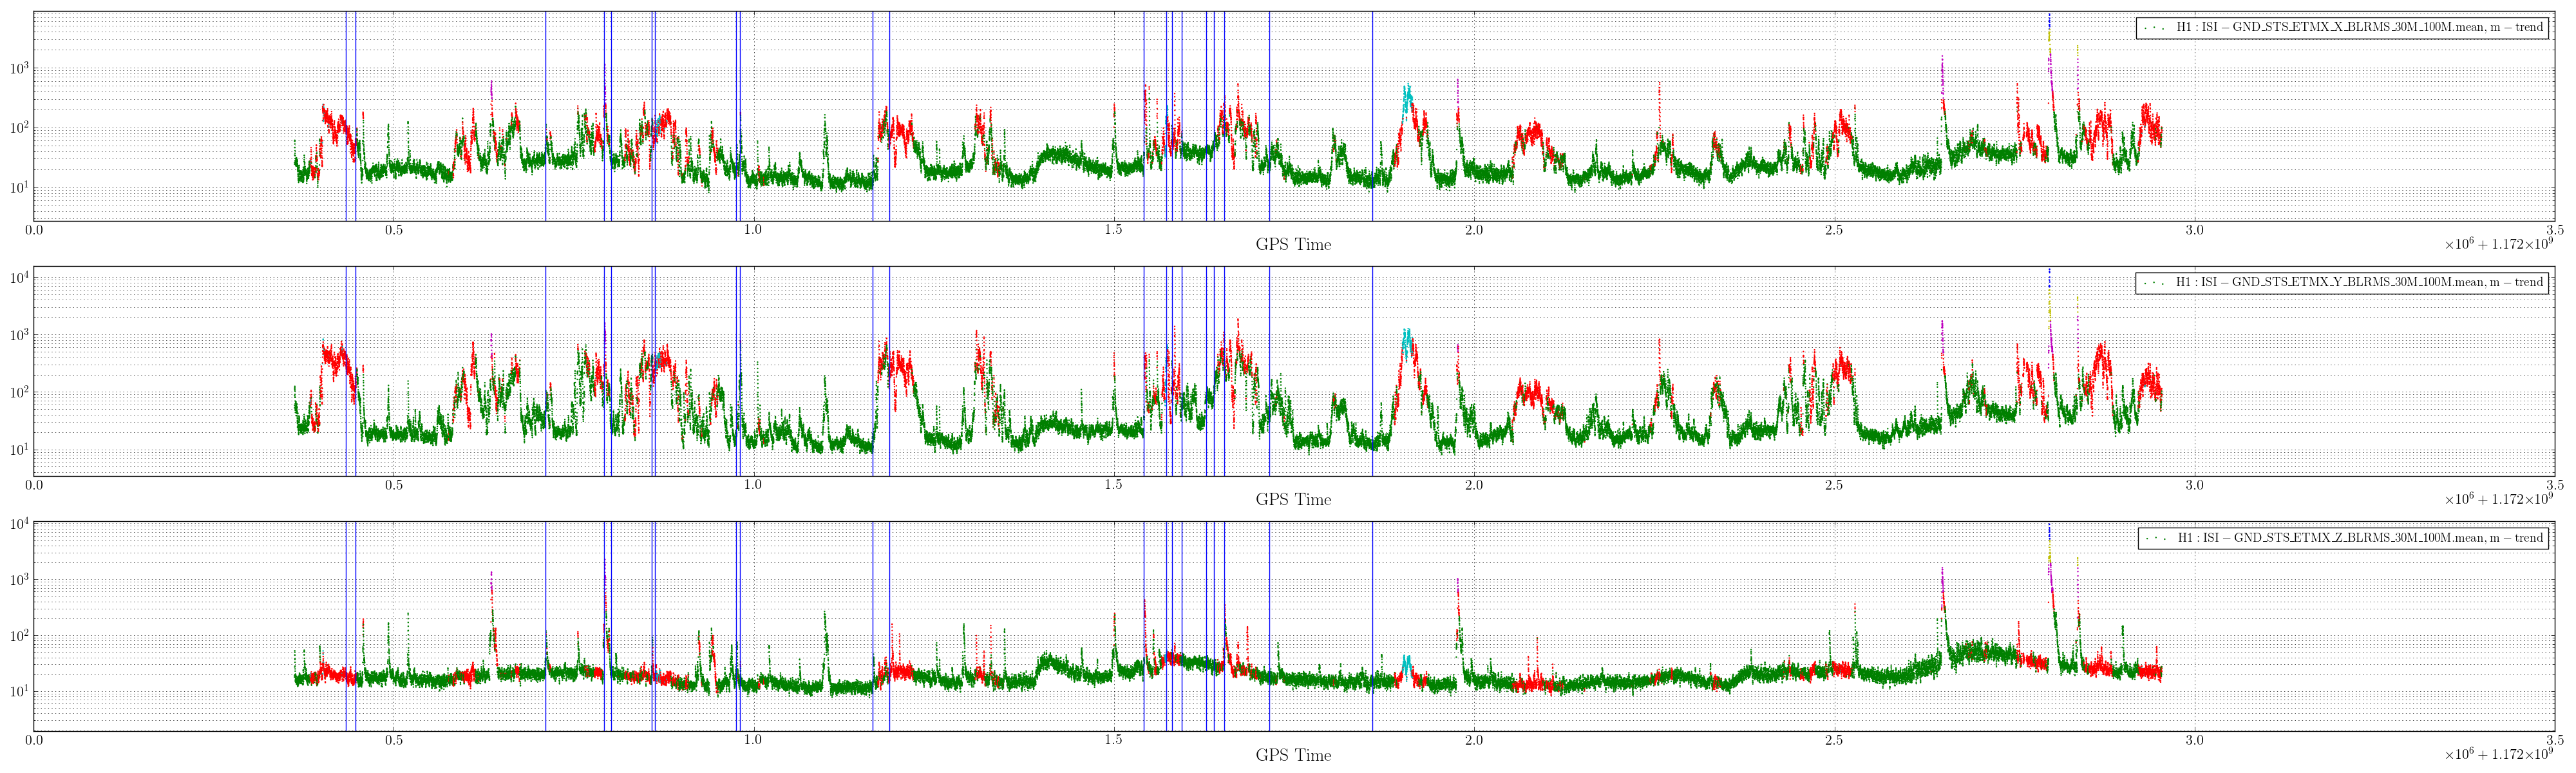
\includegraphics[width=1.3\textwidth,angle=90]{Kmeans_all6_.png}
\caption{Plot of data from earthquake channels clustered using kmeans with k=6 (earthquakes indicated)}
\label{fig:image1}
\end{center}
\end{figure}

\begin{figure}[htbp]
\begin{center}
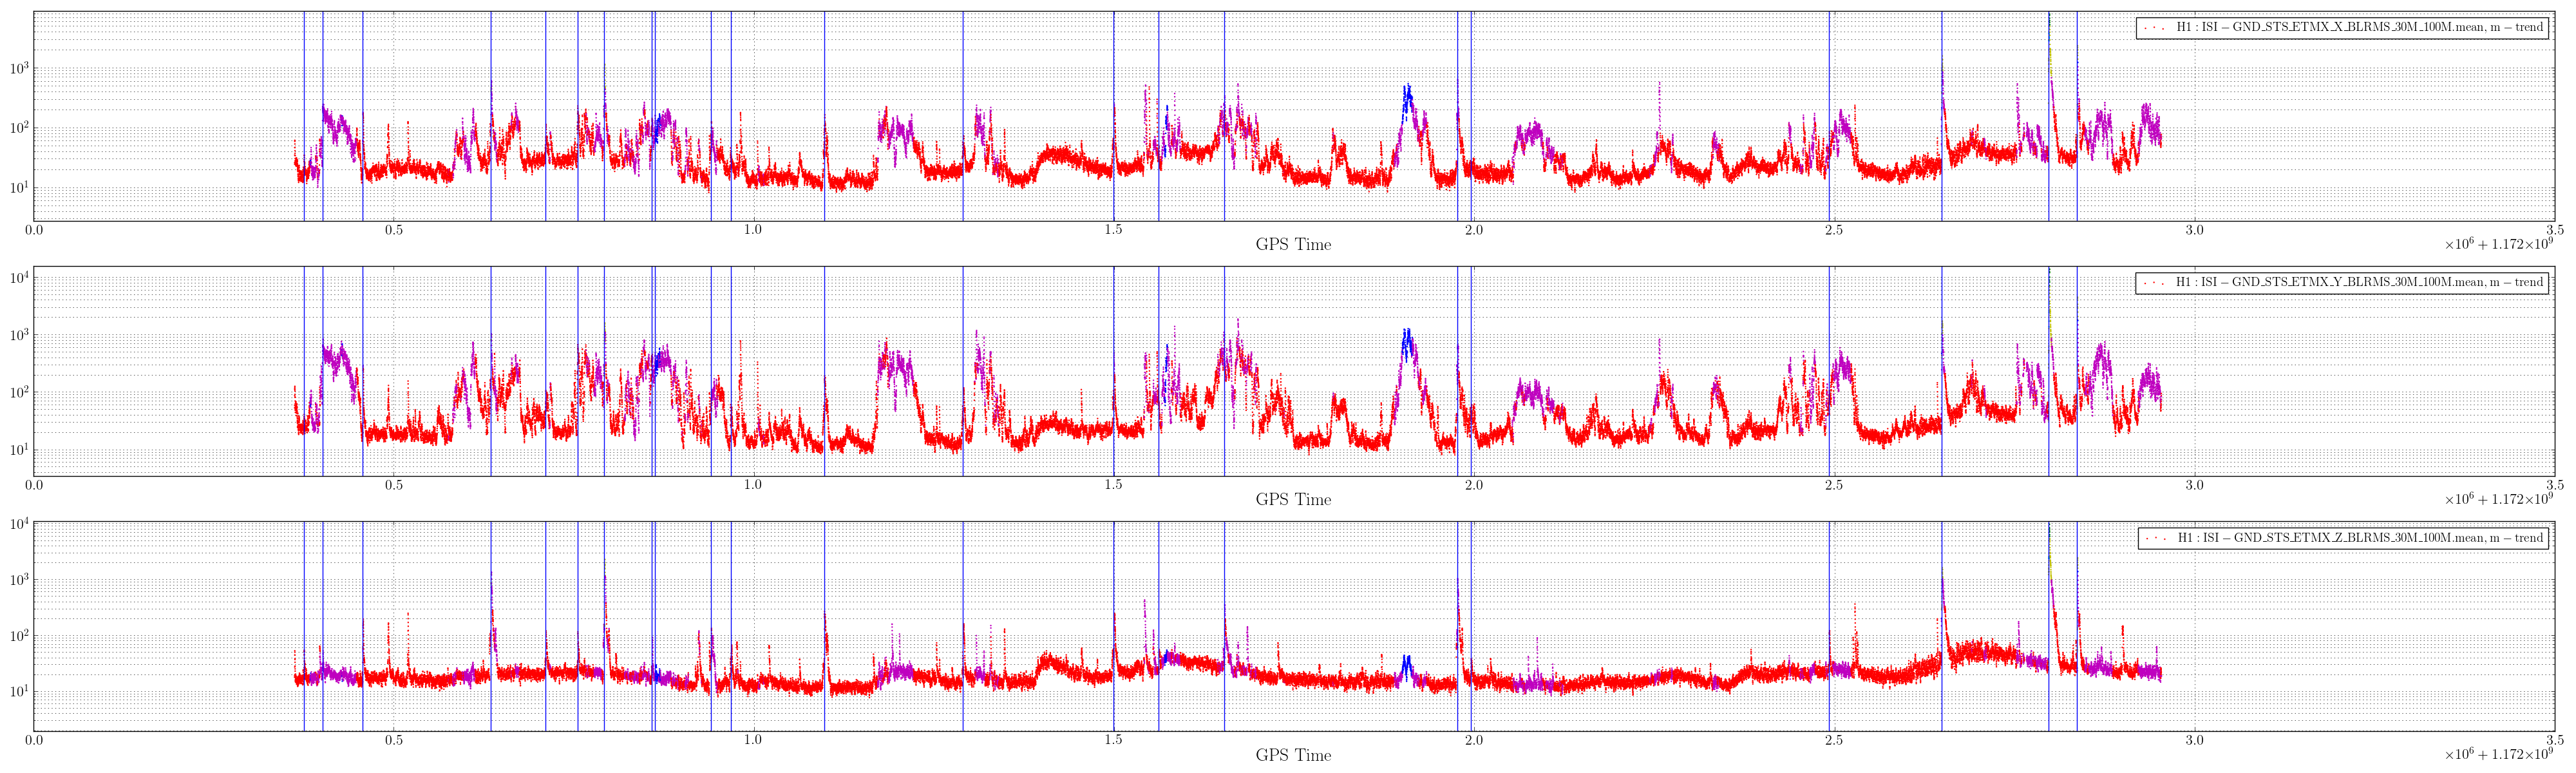
\includegraphics[width=1.3\textwidth,angle=90]{Timeshift_Kmeans_all6_.png}
\caption{Plot of data from earthquake channels clustered using kmeans with k=6 on timeshifted data (earthquakes indicated)}
\label{fig:image2}
\end{center}
\end{figure}

\begin{thebibliography}{9}
      
	\bibitem{Citation1}
	  Aurelien Geron,
	  \emph{Hands-On Machine Learning with Scikit-Learn and TensorFlow}.
	 O'Reilly Media Inc., (2017).    
      
       \bibitem{Citation2}
         \url{http://scikit-learn.org/stable/modules/clustering.html}

       \bibitem{Citation3}
         \url{https://www.cse.buffalo.edu/~jing/cse601/fa12/materials/clustering_density.pdf}
 
\end{thebibliography}


\end{document} 
